\documentclass{article}

\usepackage{float}
\usepackage{graphicx}
\usepackage[dutch]{babel}

\usepackage{hyperref}
\hypersetup{
    colorlinks=true,
    linkcolor=black,
    filecolor=blue,      
    urlcolor=blue,
    pdfpagemode=FullScreen,
}

\title{Kennisgaten}
\author{Martijn Voorwinden 1776622}
\date{10-11-2022}

\newcommand{\ls}[8]{
    \maketitle
    \section*{Kennisgaten}
    \subsection*{Inleiding}
    #1
    \subsection*{Criteria}
    \begin{itemize}
        \item Kennis opdoen en kunnen toepassen binnen context.
    \end{itemize}
    \subsection*{Learning / Research Story}
    \textbf{#2}
    % ss van story in backlog
    #3
    \subsubsection*{Acceptatiecriteria}
    % itemize
    #4
    \subsubsection*{Definition of Done (DoD)}
    % itemize
    #5
    \subsubsection*{Estimate}
    #6
    \subsubsection*{Artifacten / Realisatie}
    #7
    \subsubsection*{Bronnen}
    #8
}

\begin{document}
    \ls
    {
        Voor provincie Utrecht moet er een datacatalogus gemaakt worden om de me-
        dewerkers makkelijker toegang te geven tot de verschillende databronnen in de
        verschillende afdelingen van de provincie. Dit is nodig om te zorgen dat er geen
        dubbele datasets worden aangeschaft en om de zoektijd naar relevante datasets
        te verkleinen. Mijn rol binnen dit project is developer.
    }
    {
        Als student wil ik leren hoe ik een model bij kan houden en kan updaten in elm, 
        zodat ik interactieve website kan maken voor het project.
    }
    {
        \begin{figure}[H]
            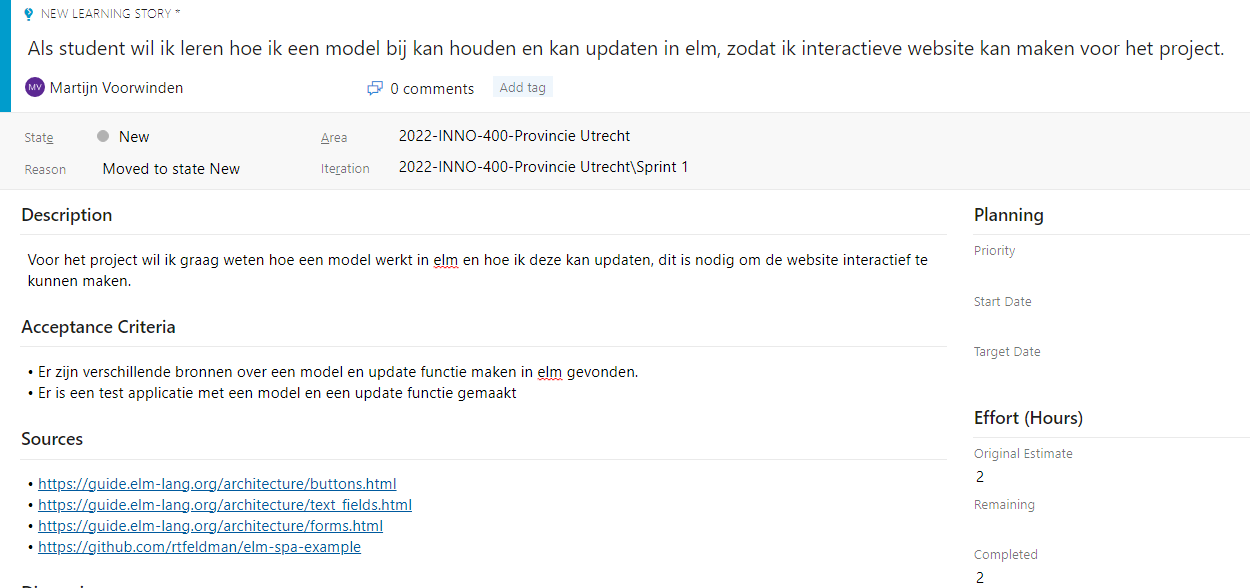
\includegraphics[width=\textwidth,height=\textheight,keepaspectratio]{ls_02.png}
            \caption{\href{https://dev.azure.com/HU-HBO-ICT/2022-INNO-400-Provincie\%20Utrecht/_backlogs/backlog/2022-INNO-400-Provincie\%20Utrecht\%20Team/Epics/?workitem=96711}{De learning story in devops.}}
            \label{fig:ls_01}
        \end{figure}
        Voor het project wil ik graag weten hoe een model werkt in elm en hoe ik deze kan updaten,
        dit is nodig om de website interactief te kunnen maken.
    }
    {
        \begin{itemize}
            \item Er zijn verschillende bronnen over een model en update functie maken in elm gevonden.
            \item Er is een test applicatie met een model en een update functie gemaakt gemaakt.
        \end{itemize}
    }
    {
        \begin{itemize}
            \item De learning story is behaald wanneer deze op niveau is.
            \item De learning is gereviewd door een medestudent.
            \item De docent gaat akkoord met het resultaat van de learning story.
        \end{itemize}
    }
    {
        De estimate voor deze learning story is 1-2 uren, dit omdat het een relatief simpel iets is.
    }
    {
        \begin{itemize}
            \item \url{https://github.com/MartijnCBV/INNO/tree/ls_02_elm_model_update/frontend}
        \end{itemize}
    }
    {
        \begin{itemize}
            \item \url{https://guide.elm-lang.org/architecture/buttons.html}
            \item \url{https://guide.elm-lang.org/architecture/text_fields.html}
            \item \url{https://guide.elm-lang.org/architecture/forms.html}
            \item \url{https://github.com/rtfeldman/elm-spa-example}
        \end{itemize}
    }
\end{document}